\documentclass{article}
%\usepackage[spanish]{babel}
\usepackage[utf8]{inputenc}
\usepackage{amssymb}
\usepackage{xcolor}
\usepackage{xspace}
\usepackage{tabularx}
\usepackage[margin=1.9cm]{geometry}
\usepackage{amsmath}
\usepackage{minted}
\usepackage{tikz}
\usetikzlibrary{arrows}

\newcommand{\cajauno}[1]{
    $
    \begin{array}{|l|}
    \hline
      #1 \\
    \hline
    \end{array}
    $
}
\newcommand{\cajados}[2]{
    $
    \begin{array}{|l|l|}
    \hline
      #1 & #2 \\
    \hline
    \end{array}
    $
}
\newcommand{\cajatres}[3]{
    $
    \begin{array}{|l|l|l|}
    \hline
      #1 & #2 & #3 \\
    \hline
    \end{array}
    $
}

\colorlet{darkgreen}{green!60!black}
\newcommand{\TODO}[1]{\textcolor{red}{TODO: #1}}
\newcommand{\HS}{\hspace{.5cm}}
\newcommand{\flecha}{\textsf{Flecha}\xspace}
\newcommand{\mamarracho}{\textsf{Mamarracho}\xspace}
\newcommand{\tok}[1]{\textcolor{red}{{\texttt{$\langle$#1$\rangle$}}}}
\newcommand{\nonterm}[1]{\textcolor{blue}{{\em{$\langle$#1$\rangle$}}}}
\newcommand{\produccion}[2]{
  \item[]
  \begin{tabularx}{\textwidth}{lrlr}
  #1 & $\xrightarrow{\hspace{.5cm}}$ & #2
  \end{tabularx}\\
}
\newcommand{\EMPTY}{$\epsilon$}
\newcommand{\ALT}{
  \\ & $\mid$ &
}

% AST
\newcommand{\type}[1]{\textcolor{darkgreen}{\texttt{#1}}}
%\renewcommand{\ast}[1]{\textcolor{darkgreen}{\texttt{\underline{#1}}}}
%\newcommand{\instruction}[1]{\textcolor{darkgreen}{\texttt{\underline{#1}}}}
\newcommand{\typedecl}[2]{\noindent
  \begin{tabularx}{\textwidth}{lrlr}
  #1 & $=$ & #2
  \end{tabularx}\\
}
\newcommand{\datadecl}[2]{\noindent
  \begin{tabularx}{\textwidth}{lrp{13cm}r}
  #1 & $::=$ & #2
  \end{tabularx}\\
}
\newcommand{\fl}[1]{\mintinline{haskell}{#1}}
\newcommand{\astkw}[1]{\texttt{\textcolor{red}{"#1"}}}
\newcommand{\astid}[1]{\texttt{"#1"}}
\newcommand{\astpart}[2]{$\underbrace{\text{#2}}_{\text{#1}}$}
\newcommand{\instruction}[1]{\texttt{\textcolor{blue}{#1}}}

\begin{document}
\begin{center}
\textsc{{\small Parseo y Generaci\'on de C\'odigo -- $2^{\text{do}}$ semestre 2018}} \medskip \\ 
\textsc{{\small Licenciatura en Inform\'atica con Orientaci\'on en Desarrollo de Software}} \medskip \\
\textsc{{\small Universidad Nacional de Quilmes}} \medskip \\
{\Large Trabajo pr\'actico 2} \medskip \\
{\large {\bf Generador de código \flecha $\to$ \mamarracho}} \medskip \\
\bigskip
Fecha de entrega: 15 de noviembre
\end{center}

\tableofcontents

\section{Introducci\'on}

Este TP consiste en implementar un generador de código
para el lenguaje de programación funcional \flecha,
extendiendo el parser ya desarrollado para el TP~1.
El lenguaje objeto será la máquina
virtual \mamarracho, diseñada {\em ad hoc} para este TP.
En la página de la materia pueden encontrar un intérprete
de \mamarracho escrito en C++.

\section{Descripción de los lenguajes}

\subsection{Lenguaje fuente (\flecha)}

La sintaxis concreta de \flecha es la que ya fue especificada e implementada en el TP~1.
En este TP el lenguaje \flecha contará con dos funciones primitivas
\texttt{unsafePrintChar} y \texttt{unsafePrintInt}
que sirven para mostrar valores en pantalla;
esto no requiere extender la gramática, pero sí
hacer algunas consideraciones.
A continuación recordamos la forma que tienen
los árboles de sintaxis abstracta de \flecha.
\bigskip

%Cada vez Los registros locales.

\noindent Un programa es una lista de definiciones: \\
\datadecl{\type{Program}}{[
  \type{Definition},
  $\hdots$,
  \type{Definition}
]
\hfill {\small Lista de $n$ definiciones, con $n \geq 0$.}
}

\noindent Cada definición asocia un identificador a una expresión: \\
\datadecl{\type{Definition}}{
[\astkw{Def}, \type{ID}, \type{Expr}]
\hfill {\small Definición.}
}

\noindent Las expresiones son las siguientes: \\
\datadecl{\type{Expr}}{
[\astkw{ExprVar}, \type{ID}]
  \hfill {\small Variable.}
\ALT
[\astkw{ExprConstructor}, \type{ID}]
  \hfill {\small Constructor.}
\ALT
[\astkw{ExprNumber}, \type{NUM}]
  \hfill {\small Constante numérica.}
\ALT
[\astkw{ExprChar}, \type{NUM}]
  \hfill {\small Constante de caracter.}
\ALT
[\astkw{ExprCase}, \type{Expr}, [\type{CaseBranch}, $\hdots$, \type{CaseBranch}]]
  \hfill {\small Case de $n$ ramas, con $n \geq 0$.}
\ALT
[\astkw{ExprLet}, \type{ID}, \type{Expr}, \type{Expr}]
  \hfill {\small Declaración local.}
\ALT
[\astkw{ExprLambda}, \type{ID}, \type{Expr}]
  \hfill {\small Función anónima.}
\ALT
[\astkw{ExprApply}, \type{Expr}, \type{Expr}]
  \hfill {\small Aplicación.}
}
\medskip

\datadecl{\type{CaseBranch}}{
  [\astkw{CaseBranch}, \type{ID}, [\type{ID}, $\hdots$, \type{ID}], \type{Expr}]
  \hfill {\small Rama del case de $n$ parámetros, con $n \geq 0$.}
}

\subsection{Lenguaje objeto (\mamarracho)}

\noindent
El generador de código debe producir código para la máquina virtual
\mamarracho.
Al momento de la ejecución, el estado de \mamarracho consta de:
\begin{enumerate}
\item El {\bf código fuente}, que es una secuencia de instrucciones,
      incluyendo definiciones de etiquetas.
\item El {\bf puntero a la instrucción actual}.
\item Un {\bf entorno global} que le da valor a los registros globales.
\item Un {\bf entorno local} que le da valor a los registros locales.
\item Una {\bf memoria} indexada por enteros de 64 bits.
\item Una {\bf pila de llamadas} en la que se guardan las locaciones
      de retorno y el entorno local cada vez que se invoca a una
      función con las instrucciones \instruction{call}/\instruction{icall}.
\end{enumerate}
En cada posición de memoria hay una {\bf celda} de memoria.
Una celda de memoria tiene espacio para guardar $n$ {\bf slots} numerados desde $0$ hasta $n-1$.
Cada {\em slot} almacena un {\bf valor}.
Usamos \type{Val} para representar el tipo de los valores.
Los valores pueden ser:
\begin{enumerate}
\item {\bf constantes numéricas}: enteros con signo de 64 bits,
\item {\bf punteros} a celdas de memoria,
\item {\bf locaciones}, que representan una posición dentro del código fuente
      del programa.
\end{enumerate}
Más precisamente, el tipo de los valores \type{Val} está dado por:\medskip

\datadecl{\type{Val}}{
  \texttt{VInt}(\type{i64})
  \hfill {\small donde \type{i64} representa un entero con signo de 64 bits}
\ALT
  \texttt{VPtr}(\type{u64})
  \hfill {\small donde \type{u64} representa un entero sin signo de 64 bits}
\ALT
  \texttt{VLoc}(\type{u64})
}

\bigskip
La máquina virtual cuenta con un número ilimitado
de {\bf registros globales}
(\texttt{@r1}, \texttt{@r2}, \texttt{@r3}, $\hdots$)
y {\bf registros locales}
(\texttt{\$r1}, \texttt{\$r2}, \texttt{\$r3}, $\hdots$).
El nombre de un registro es un identificador arbitrario\footnote{Con
la sintaxis léxica \texttt{[\_a-zA-Z][\_a-zA-Z0-9]*}.}
que comienza con arroba (\texttt{@}) para los registros globales
y con el signo pesos (\texttt{\$}) para los registros locales.
Usamos \type{Reg} para representar el tipo de los registros.
Cada registro puede almacenar un valor.
Si $r$ es un registro en el que hay almacenado un puntero \texttt{$p$}
a una celda de memoria con $n$ slots,
escribimos $r[i]$ para denotar el valor almacenado en el $i$-ésimo slot de la celda
apuntada por $p$, para cada $0 \leq i < n$.
La semántica informal se describe al costado de cada instrucción:
\bigskip

\datadecl{\type{Instruction}}{
  \instruction{mov\_reg}($r_1$ : \type{Reg}, $r_2$ : \type{Reg})
  \hfill {\small $r_1 := r_2$}
\ALT
  \instruction{mov\_int}($r$ : \type{Reg}, $n$ : \type{i64})
  \hfill {\small $r := \texttt{VInt}(n)$}
\ALT
  \instruction{mov\_label}($r$ : \type{Reg}, $l$ : \type{Label})
  \hfill {\small $r := \texttt{VLoc}(p)$, donde $p$ es la locación} \\
  && \hfill {\small de la etiqueta $l$ en el código fuente}
\ALT
  \instruction{alloc}($r$ : \type{Reg}, $n$ : \type{u64})
  \hfill {\small $r := \texttt{VPtr}(p)$, donde $p$ es un puntero a una} \\
  && \hfill {\small celda de memoria nueva con $n$ slots}
\ALT
  \instruction{load}($r_1$ : \type{Reg}, $r_2$ : \type{Reg}, $i$ : \type{u64})
  \hfill {\small $r_1 := r_2[i]$}
\ALT
  \instruction{store}($r_1$ : \type{Reg}, $i$ : \type{u64}, $r_2$ : \type{Reg})
  \hfill {\small $r_1[i] := r_2$}
\ALT
  \instruction{print}($r$ : \type{Reg})
  \hfill {\small Imprime en la salida el valor almacenado en $r$.}
\ALT
  \instruction{print\_char}($r$ : \type{Reg})
  \hfill {\small Imprime en la salida el caracter almacenado en $r$.}
\ALT
  \instruction{jump}($l$ : \type{Label})
  \hfill {\small Salta a $l$.}
\ALT
  \instruction{jump\_eq}($r_1$ : \type{Reg}, $r_2$ : \type{Reg}, $l$ : \type{Label})
  \hfill {\small Si $r_1 == r_2$, salta a $l$.}
\ALT
  \instruction{jump\_lt}($r_1$ : \type{Reg}, $r_2$ : \type{Reg}, $l$ : \type{Label})
  \hfill {\small Si $r_1 < r_2$, salta a $l$.}
\ALT
  \instruction{add}($r_1$ : \type{Reg}, $r_2$ : \type{Reg}, $r_3$ : \type{Reg})
  \hfill {\small $r_1 := r_2 + r_3$}
\ALT
  \instruction{sub}($r_1$ : \type{Reg}, $r_2$ : \type{Reg}, $r_3$ : \type{Reg})
  \hfill {\small $r_1 := r_2 - r_3$}
\ALT
  \instruction{mul}($r_1$ : \type{Reg}, $r_2$ : \type{Reg}, $r_3$ : \type{Reg})
  \hfill {\small $r_1 := r_2 * r_3$}
\ALT
  \instruction{div}($r_1$ : \type{Reg}, $r_2$ : \type{Reg}, $r_3$ : \type{Reg})
  \hfill {\small $r_1 := r_2 \texttt{ div } r_3$}
\ALT
  \instruction{mod}($r_1$ : \type{Reg}, $r_2$ : \type{Reg}, $r_3$ : \type{Reg})
  \hfill {\small $r_1 := r_2 \texttt{ mod } r_3$}
\ALT
  \instruction{call}($l$ : \type{Label})
  \hfill {\small Guarda la dirección de retorno y el entorno local actual en la pila.} \\
  && \hfill {\small Crea un nuevo entorno local y salta a la locación de la etiqueta $l$.}
\ALT
  \instruction{icall}($r$ : \type{Reg})
  \hfill {\small Similar a \instruction{call}, pero salta a la locación almacenada en $r$.}
\ALT
  \instruction{return}()
  \hfill {\small Restaura la dirección de retorno y el entorno local de la pila,}
  \\
  && \hfill {\small retornando a la posición del último \instruction{call}/\instruction{icall}.}
}

\medskip
Notar que 
para poder pasar parámetros y devolver resultados de funciones
se deben utilizar los registros globales,
ya que cuando se ejecuta una instrucción
\instruction{call}/\instruction{icall}
se crea un nuevo entorno local.
\medskip

Un programa es una lista de instrucciones
y declaraciones de etiquetas. Una declaración de etiqueta es de la forma
``\texttt{etiqueta:}''. Por ejemplo, el siguiente programa en \mamarracho
imprime diez veces el número 9 en la salida:

\begin{verbatim}
  mov_int($actual, 0)
  mov_int($limite, 10)
  mov_int($uno, 1)
  mov_int($valor, 9)
iniciar_loop:
  jump_lt($actual, $limite, continuar_loop)
  jump(fin_loop)
continuar_loop:
  print($valor)
  add($actual, $actual, $uno)
  jump(iniciar_loop)
fin_loop:
\end{verbatim}

\section{Estructura del compilador}

\subsection{Representación de los datos}

Todos los valores del lenguaje \flecha (enteros, caracteres, funciones y
estructuras de datos armadas con constructores)
se representan con celdas de memoria del lenguaje \mamarracho.
El primer slot de la celda es siempre un entero
que sirve como un {\bf tag} para indicar qué clase de valor se encuentra
almacenado en esa celda.  Cada constructor que aparezca en el código
fuente tendrá asociado un tag único.

Reservaremos un tag para representar valores de tipo \fl{Int},
un tag para representar valores de tipo \fl{Char},
y un tag para representar funciones (clausuras).
La primera etapa del compilador consiste en un recorrido del AST
para recolectar el conjunto de todos los constructores que aparezcan
en el código fuente del programa y armar una tabla de tags.
Por ejemplo, si en el código fuente del programa aparecen los
constructores \fl{True}, \fl{False}, \fl{Nil} y \fl{Cons}, el
compilador podría generar la siguiente tabla de tags:
\[
\begin{array}{l|l}
\text{Constructor}               & \text{tag} \\
\hline
\text{número entero (\fl{Int})}  & 1 \\
\text{caracter (\fl{Char})}      & 2 \\
\text{clausura (\fl{Closure})}   & 3 \\
\fl{True}                        & 4 \\
\fl{False}                       & 5 \\
\fl{Nil}                         & 6 \\
\fl{Cons}                        & 7 \\
\end{array}
\]
Así, por ejemplo, el valor \texttt{Cons 'A' (Cons 'B' Nil)}
se podría representar con el siguiente conjunto de celdas:
\[
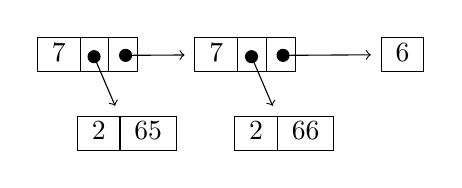
\begin{tikzpicture}
  \node (consa) at (0,0)  {\cajatres{7}{}{}};
  \node (consb) at (2,0)  {\cajatres{7}{}{}};
  \node (nil)   at (4,0)  {\cajauno{6}};
  \node (a)     at (0.5,-1) {\cajados{2}{65}};
  \node (b)     at (2.5,-1) {\cajados{2}{66}};
  \path [*->] (consa.center)+(.05,.05) edge (a);
  \path [*->] (consa.center)+(.4,-.01) edge (consb);
  \path [*->] (consb.center)+(.05,.05) edge (b);
  \path [*->] (consb.center)+(.4,-.01) edge (nil);
\end{tikzpicture}
\]

Asumiremos que cada constructor del lenguaje \flecha
se utiliza siempre con la misma cantidad de argumentos,
tanto en las aplicaciones como en las ramas de un case.
Por ejemplo, en el siguiente programa el constructor \fl{Nil}
se utiliza con aridad 0, y el constructor \fl{Cons} se utiliza
con aridad 2:
\begin{minted}{haskell}
def longitud l = case l
                 | Nil       -> 0
                 | Cons x xs -> 1 + longitud l
def lista = Cons 1 (Cons 2 (Cons 3 Nil))
\end{minted}
Observar que esta restricción prohíbe utilizar constructores aplicados
parcialmente; por ejemplo, en dicho programa sería incorrecto
escribir una expresión como
\fl{(map (Cons 1) lista)} porque en esa expresión el constructor \fl{Cons}
se utiliza con aridad 1.
Es opcional (pero recomendable) que el compilador verifique que
todas las ocurrencias de un constructor tengan siempre la misma aridad.


\subsection{Guía de compilación}

Recordemos que un programa en \flecha consta de una lista de definiciones:
$[\astkw{Def}, x_1, e_1], ..., [\astkw{Def}, x_n, e_n]$
de constantes y funciones globales.
En el momento de la compilación,
a cada uno de los nombres {\bf globales} $x_i$ del programa
le atribuiremos un registro global $\texttt{@G\_}x_i$ en \mamarracho.
Por ejemplo, si el programa define una constante global
``\fl{def misMejoresAmigos = ...}'' su valor quedará almacenado en
el registro \texttt{@G\_misMejoresAmigos}.

Para compilar un programa de la forma
$[\astkw{Def}, x_1, e_1], ..., [\astkw{Def}, x_n, e_n]$
el compilador genera código para calcular el valor de la expresión $e_i$
y almacenar ese valor en el registro $\texttt{\$G\_}x_i$,
para todo $i=1..n$.
El ``corazón'' del compilador es una función recursiva
que recibe un entorno,
una expresión arbitraria $e$ del lenguaje \flecha,
y un registro arbitrario $r$,
y genera una secuencia de instrucciones en lenguaje \mamarracho
que calculan el valor de la expresión $e$ y almacenan su resultado en
el registro $r$.
El tipo de dicha función será algo como:
\begin{verbatim}
  compilarExpresion :: Env -> Expr -> Reg -> [Instruccion]
\end{verbatim}
Donde \texttt{Env} representa un {\bf entorno}.
Un entorno es un diccionario que indica
dónde se encuentra almacenado el valor de cada variable
del lenguaje \flecha.
Más precisamente, \texttt{Env} es un diccionario que asocia nombres
de variables a \texttt{Binding}s. Hay dos posibles formas de {\em binding}:
\[
\datadecl{\type{Binding}}{
  \texttt{BRegister}(\type{Reg})
\ALT
  \texttt{BEnclosed}(\type{Int})
}
\]
Una asociación de la forma $x \mapsto \texttt{BRegister}(r)$
representa que la variable $x$ de \flecha se encuentra guardada en el
registro $r$ de \mamarracho.
El entorno se inicializa con todas las variables globales ligadas a registros,
por ejemplo:
\[
  \{
  \texttt{main} \mapsto \texttt{BRegister}(\texttt{\$G\_main}),
  \texttt{foo} \mapsto \texttt{BRegister}(\texttt{\$G\_foo})
  \}
\]
Cada vez que se introduce una definición de variable local
el entorno se extiende asociando esa variable a un registro que no haya
sido utilizado previamente.
El {\em binding} \texttt{BEnclosed($i$)} es necesario para las variables
almacenadas en una clausura léxica, como veremos más adelante. 

\subsubsection{Caracteres}

Nuestro primer objetivo será compilar el siguiente programa:
\begin{minted}{haskell}
    def main = unsafePrintChar 'A'
\end{minted}

Para compilar un caracter, es decir una expresión $[\astkw{ExprChar}, n]$, se debe:
\begin{itemize}
\item Crear una celda de dos slots usando la instrucción \instruction{alloc}.
\item Guardar el tag para el tipo \fl{Char} en el primer slot usando la instrucción \instruction{store}.
\item Guardar $n$ en el segundo slot usando la instrucción \instruction{store}.
\end{itemize}

Para compilar la expresión \fl{(unsafePrintChar e)}, es decir
cualquier expresión que tenga esta forma:
\[
  [\astkw{ExprApply}, [\astkw{ExprVar}, \astid{unsafePrintChar}], e]
\]
\begin{itemize}
\item Compilar recursivamente la expresión $e$ en el registro $r$
\item Cargar el segundo slot usando la instrucción \instruction{load}.
\item Mostrar el caracter en pantalla usando la instrucción \instruction{print\_char}.
\end{itemize}
El programa compilado podría quedar así: 
\begin{verbatim}
  alloc($r0, 2)           % Reservar una celda de dos slots.
  mov_int($t, 2)          % 2 = tag para el tipo Char.
  store($r0, 0, $t)
  mov_int($t, 65)         % 65 = letra 'A'
  store($r0, 1, $t)
  load($r1, $r0, 1)
  print_char($r1)
  mov_reg @G_main, $r0    % Guardar en @G_main el valor del caracter.
\end{verbatim}

\subsubsection{Números enteros}

Se compilan de manera similar a los caracteres.
El lenguaje incluye una primitiva 
\fl{(unsafePrintInt e)}
que se debe compilar usando la instrucción \instruction{print}.

% Nuestro segundo objetivo será compilar el siguiente programa:
% \begin{minted}{haskell}
%     def main = unsafePrintInt 42
% \end{minted}
% 
% Para compilar un entero, es decir una expresión $[\astkw{ExprNumber}, n]$
% el procedimiento es parecido al de compilar un caracter:
% \begin{itemize}
% \item Crear una celda de dos slots usando la instrucción \instruction{alloc}.
% \item Guardar el tag para el tipo \fl{Int} en el primer slot usando la instrucción \instruction{store}.
% \item Guardar $n$ en el segundo slot usando la instrucción \instruction{store}.
% \end{itemize}
% 
% Para compilar la expresión \fl{(unsafePrintInt e)}, es decir
% cualquier expresión que tenga esta forma:
% \[
%   [\astkw{ExprApply}, [\astkw{ExprVar}, \astid{unsafePrintInt}], e]
% \]
% \begin{itemize}
% \item Compilar recursivamente la expresión $e$ en el registro $r$
% \item Cargar el segundo slot usando la instrucción \instruction{load}.
% \item Mostrar el número en pantalla usando la instrucción \instruction{print}.
% \end{itemize}
% El programa compilado podría quedar así:
% \begin{verbatim}
%   alloc($r0, 2)           % reservar una celda de 2 slots
%   mov_int($t, 1)          % 1 = tag para el tipo Int
%   store($r0, 0, $t)
%   mov_int($t, 42)
%   store($r0, 1, $t)
%   load($r1, $r0, 1)
%   print($r1)
%   mov_reg $G_main, $r0    % guardar en $G_main el valor del entero
% \end{verbatim}

\subsubsection{Constructor aislado}

Un constructor aislado (de aridad 0)
se debe compilar como una celda de memoria
con un único slot que contiene el tag del constructor.
Por ejemplo, para compilar el constructor \texttt{True}:
\begin{verbatim}
  alloc($r, 1)           % Reservar una celda de 1 slot.
  mov_int($t, 4)         % 4 = Tag para el constructor True.
  store($r, 0, $t)
\end{verbatim}

\subsubsection{Variables}

Para compilar una variable $[\astkw{ExprVar}, x]$,
se debe buscar en el entorno de qué manera está ligada.

Si la variable está ligada a \texttt{BRegister($r$)},
significa que está almacenada en el registro $r$. En ese caso,
se debe copiar el contenido de dicho registro al registro objetivo,
usando la instrucción \instruction{mov\_reg}.
Por ejemplo, el resultado de compilar:
\begin{minted}{haskell}
def foo = 42
def main = unsafePrintInt foo
\end{minted}
podría ser el siguiente código:
\begin{verbatim}
  % Código para "def foo = 42":
  alloc($r0, 2)
  mov_int($t, 1)
  store($r0, 0, $t)
  mov_int($t, 42)
  store($r0, 1, $t)
  mov_reg(@G_foo, $r0)

  % Código para "def main = unsafePrintInt foo":
  mov_reg($r1, @G_foo)
  load($r2, $r1, 1)
  print($r2)
  mov_reg(@G_main, $r1)
\end{verbatim}

Por otro lado,
si una variable está ligada en el entorno a \texttt{BEnclosed($i$)},
esto significa que la variable se encuentra almacenada en una
clausura léxica. Más adelante se describe cómo compilar una variable
en este caso.

\subsubsection{Declaraciones locales (let)}

Para compilar una declaración local $[\astkw{ExprLet}, x, e_1, e_2]$:
\begin{itemize}
\item Reservar un registro fresco $\$tmp$.
\item Compilar $e_1$ guardando su valor en $\$tmp$.
\item Compilar $e_2$ en el entorno extendido con la asociación
      $x \mapsto \$tmp$.
\end{itemize}
Observar que el lenguaje tiene semántica {\em call-by-value}
porque $e_1$ se evalúa siempre antes que $e_2$.

\subsubsection{Funciones anónimas ($\lambda$)}

Un programa \flecha compilado se organiza como un conjunto de rutinas
auxiliares seguido de la rutina principal.
Cada rutina está encabezada por una etiqueta
($\texttt{rtn}_1$, $\texttt{rtn}_2$, $\hdots$, $\texttt{rtn}_m$):
\begin{verbatim}
  jump start
  rtn_1:
    <rutina 1>
  rtn_2:
    <rutina 2>
  ...
  rtn_m:
    <rutina m>
  start:
    <programa>
\end{verbatim}
A cada función anónima que aparece en el código fuente le corresponde una
rutina $\texttt{rtn}_i$.
Una función anónima $[\astkw{ExprLambda}, x, e]$ se compila como una
{\bf clausura léxica}. Una clausura es una celda de memoria con $2 + n$ slots.
En el primer slot se almacena el tag clausura.
En el segundo slot se almacena la locación de la rutina $\texttt{rtn}_i$.
En los $n$ slots restantes, se guardan los valores de todas
las variables libres de aparecen en $e$ (excluyendo el parámetro $x$,
los nombres de las constantes globales definidas en el programa
como \texttt{misMejoresAmigos},
y las primitivas como \texttt{unsafePrintChar} o \texttt{ADD}).
A dichas $n$ variables $a_1,a_2,\hdots,a_n$ las llamamos
{\bf variables clausuradas}.

Por ejemplo, el código para una función \fl{(\ x -> e)} en la que aparecen
tres variables libres \fl{a}, \fl{b} y \fl{c} será algo como lo siguiente:
\begin{verbatim}
  alloc($r, 5)       % Reservar una celda con 5 slots (5 = 2 + 3).
  mov_int($t, 3)
  store($r, 0, $t)   % Guardar el tag "clausura" en $r[0].
  mov_label($t, rtn_i)
  store($r, 1, $t)   % Guardar la rutina rtn_i en $r[1].
  <guardar en $t el valor de la variable "a">
  store($r, 2, $t)
  <guardar en $t el valor de la variable "b">
  store($r, 3, $t)
  <guardar en $t el valor de la variable "c">
  store($r, 4, $t)
\end{verbatim}

Todas las rutinas reciben exactamente dos parámetros en los registros
globales \texttt{@fun} y \texttt{@arg},
y devuelven exactamente un resultado en el registro \texttt{@res}.
La rutina $\texttt{rtn}_i$ tiene la siguiente estructura:
\begin{verbatim}
  rtn_i:
    mov_reg($fun, @fun)    % Mover el parámetro @fun a un registro local.
    mov_reg($arg, @arg)    % Mover el parámetro @arg a un registro local.
    % Ejecutar el cuerpo de la función y guardar
    % el resultado en un registro local $res.
    <código compilado para el cuerpo de la función>
    mov_reg(@res, $res)    % Mover el resultado al registro global @res.
    return()
\end{verbatim}

\noindent{\bf Acceso a parámetros y variables clausuradas.}
Cuando se compila el cuerpo $e$ de una función \fl{(\ x -> e)},
se debe extender el entorno del siguiente modo:
\begin{itemize}
\item El parámetro $x$ debe quedar ligado a \texttt{BRegister(\$arg)}.
      Es decir, el valor del parámetro $x$ se encuentra inmediatamente
      en el registro local \texttt{\$arg}.
\item Si las variables clausuradas son $a_1,a_2,\hdots,a_n$
      el valor de la $i$-ésima variable clausurada se encuentra
      en el slot \texttt{\$fun[i + 2]}. Por ejemplo, si se quiere
      recuperar el valor de $a_3$ y guardarlo en el registro \texttt{\$r}
      se utilizará la siguiente instrucción:
\begin{verbatim}
  load($r, $fun, 5)
\end{verbatim}
      Para ello se registrará en el entorno que (para cada $i=1..n$)
      la variable $a_i$ se encuentra ligada a \texttt{BEnclosed($i$)}.
\end{itemize}

\subsubsection{Aplicación (caso típico)}

Empezamos describiendo cómo compilar una
aplicación \texttt{[\astkw{ExprApply}, $e_1$, $e_2$]}
en el caso típico.
En tal caso, el resultado de evaluar $e_1$ es una clausura. 
El código será como el siguiente:

\begin{verbatim}
  <evaluar e1 y guardar el valor en un registro temporal $r1>
  <evaluar e2 y guardar el valor en un registro temporal $r2>
  load($r3, $r1, 1)   % Cargar la locación de la clausura en $r3.
  mov_reg(@fun, $r1)  % Pasar e1 como parámetro en el registro global @fun.
  mov_reg(@arg, $r2)  % Pasar e2 como parámetro en el registro global @arg.
  icall($r3)          % Invocar.
  mov_reg($r, @res)   % Obtener el resultado del registro global @res.
\end{verbatim}

\subsubsection{Aplicación (constructor)}

Si en una aplicación \texttt{[\astkw{ExprApply}, $e_1$, $e_2$]}
la función $e_1$ es un constructor posiblemente aplicado a argumentos
(por ejemplo, $e_1 = \texttt{(Cons 1)}$ y $e_2 = \texttt{Nil}$),
debemos proceder de otra manera.
En general,
tendremos un constructor \texttt{C} aplicado a $n$ expresiones:
$\texttt{C}\ e_1\ \hdots\ e_n$ y se debe generar código para
construir una celda de memoria de $1+n$ slots,
donde el primer slot corresponde al tag del constructor. 
Por ejemplo, para $\texttt{Cons}\ e_1\ e_2$
generaremos:

\begin{verbatim}
  <evaluar e1 y guardar el valor en un registro temporal $r1>
  <evaluar e2 y guardar el valor en un registro temporal $r2>
  alloc($r, 3)
  mov_int($t, 7)     % 7 = tag para el constructor Cons.
  store($r, 0, $t)
  store($r, 1, $r1)
  store($r, 2, $r2)
\end{verbatim}

\subsubsection{{\em Pattern matching} (\texttt{case})}

Para compilar un \texttt{case} de la forma $[\astkw{ExprCase}, expr, ramas]$.
se debe, en primer lugar compilar la expresión $e$ guardando el resultado
en un registro temporal \texttt{\$val}.
Supongamos que el case cuenta con $n$ ramas,
cuyos constructores son $\texttt{C}_1, \texttt{C}_2, \hdots, \texttt{C}_n$,
y que los tags de dichos constructores son
$\texttt{TAG}_1, \texttt{TAG}_2, \hdots, \texttt{TAG}_n$,
respectivamente.
El case compilado tiene la forma siguiente:

\begin{verbatim}
  <evaluar expr y guardar el valor en un registro temporal $val>
  load($tag, $val, 0)           % Obtener el tag del valor analizado.
  mov_int($test, <TAG_1>)
  jump_eq($tag, $test, RAMA_1)  % Si el tag es TAG_1 saltar a la rama 1.
  mov_int($test, <TAG_2>)
  jump_eq($tag, $test, RAMA_2)  % Si el tag es TAG_2 saltar a la rama 2.
  ...
  mov_int($test, <TAG_n>)
  jump_eq($tag, $test, RAMA_n)  % etc.

  RAMA_1: <código para la rama 1> jump FIN_CASE
  RAMA_2: <código para la rama 2> jump FIN_CASE
  ...
  RAMA_n: <código para la rama n> jump FIN_CASE
  FIN_CASE:
\end{verbatim}
Las etiquetas $\texttt{RAMA}_1, \hdots, \texttt{RAMA}_n$ y \texttt{FIN\_CASE}
son etiquetas frescas.
\bigskip

Para compilar una rama de la forma
$[\astkw{CaseBranch}, constructor, [x_1, \hdots, x_n], e]$,
se deben recuperar los $n$ argumentos del constructor
que se encuentran almacenados la celda de memoria referenciada
por \texttt{\$val}, usando la instrucción \instruction{load}.
El $i$-ésimo argumento del constructor se guarda en un registro
temporal $\texttt{\$r}_i$,
y se compila la expresión $e$ en el entorno extendido
con $\{
  x_1 \mapsto \texttt{BRegister}(\texttt{\$r}_1),
  \hdots,
  x_n \mapsto \texttt{BRegister}(\texttt{\$r}_n)
\}$

\subsubsection{Aplicación (primitiva)}
Si en una aplicación \texttt{[\astkw{ExprApply}, $e_1$, $e_2$]}
la función es una primitiva aplicada {\bf exactamente} al número de
argumentos que recibe
(por ejemplo, $e_1 = \texttt{(ADD 11)}$ y $e_2 = \texttt{31}$)
se debe emitir código para calcular la primitiva en cuestión.

Se deja como ejercicio opcional
completar la implementación de todas las
primitivas que reconoce el parser del TP~1:
\texttt{OR},
\texttt{AND},
\texttt{NOT},
\texttt{EQ},
\texttt{NE},
\texttt{GE},
\texttt{LE},
\texttt{GT},
\texttt{LT},
\texttt{ADD},
\texttt{SUB},
\texttt{MUL},
\texttt{DIV},
\texttt{MOD},
\texttt{UMINUS}.

\section{Pautas de entrega}

Para entregar el TP se debe enviar el c\'odigo fuente por e-mail
a la casilla \texttt{foones@gmail.com} hasta las 23:59:59 del d\'ia
estipulado para la entrega, incluyendo \texttt{[TP lds-est-parse]} en
el asunto y el nombre de los integrantes del grupo en el cuerpo
del e-mail. No es necesario hacer un informe sobre el TP, pero se espera
que el c\'odigo sea razonablemente legible.
Se debe incluir un README
indicando las dependencias y el mecanismo de ejecuci\'on
recomendado para que el programa provea la funcionalidad pedida.
Se recomienda probar el programa con el conjunto de tests provistos.

\end{document}

